\documentclass[10pt,aspectratio=169]{beamer}
\usetheme{Madrid}
\usecolortheme{default}
\usepackage{graphicx}
\usepackage{booktabs}
\graphicspath{{../figures/}}
\setbeamertemplate{navigation symbols}{}
\setbeamerfont{caption}{size=\scriptsize}

\definecolor{unairblue}{RGB}{42,120,214}

\title{An AI-Based Materials Informatics Framework for the Discovery of Calcium Phosphate Scaffold Candidates}
\author[Soelistiono et al.]{Soegianto Soelistiono, Herri Trilaksana, Yhosep G. Y. Yhuwana, Bernardi Pranggono}
\institute[AMREC -- Universitas Airlangga]{Advanced Materials and Renewable Energy Conversion (AMREC)\\ Universitas Airlangga -- Anglia Ruskin University}
\date{November 2026}

\begin{document}

\begin{frame}
\titlepage
\end{frame}

\begin{frame}{Motivation}
\begin{itemize}
\item Bone defects from trauma, degenerative disease, congenital abnormalities remain a major clinical challenge.
\item Calcium phosphates (CaP) are biocompatible, bioactive, osteoconductive --- the scaffold materials of choice.
\item Conventional trial-and-error discovery is slow and costly.
\item \textbf{Goal:} an end-to-end, replicable Materials Informatics framework that accelerates CaP scaffold discovery with AI.
\end{itemize}
\end{frame}

\begin{frame}{Framework workflow}
\centering
Data Mining $\rightarrow$ Preprocessing $\rightarrow$ Descriptors $\rightarrow$ EDA/Clustering $\rightarrow$ ML $\rightarrow$ MCDM $\rightarrow$ XAI\\[2mm]
\begin{tabular}{lll}
\toprule
Stage & Tools & Output \\
\midrule
Acquisition & 5 open databases & 2{,}885 entries / 950 compositions \\
Preprocessing & QC, IQR/z-score & audited dataset \\
Descriptors & Ca/P, EN, VEC, cell volume, density & 10 descriptors \\
EDA & PCA, t-SNE, UMAP, K-Means, HDBSCAN & design-space map \\
ML & SVR, RF, XGBoost (GroupKFold) & $R^2$ up to 0.91 \\
MCDM & TOPSIS + VIKOR $\times$ 3 weights & Top-15 candidates \\
XAI & SHAP & descriptor roles \\
\bottomrule
\end{tabular}
\end{frame}

\begin{frame}{Dataset: 5 open sources}
\begin{table}
\centering
\begin{tabular}{llcl}
\toprule
Source & Access & License & Entries \\
\midrule
Materials Project & API key & CC-BY 4.0 & 57 \\
AFLOW (AFLUX) & REST & cite Curtarolo et al. & 234 \\
COD & HTTP & CC0 & 2{,}304 \\
PubChem & PUG REST & public domain & 13 \\
OQMD & oqmdapi & cite Kirklin et al. & 280 \\
\midrule
\textbf{Total} & & & \textbf{2{,}885} \\
\bottomrule
\end{tabular}
\caption{950 unique compositions (target $\geq$500 met); cell volume \& space group 99.5\% complete.}
\end{table}
\end{frame}

\begin{frame}{Design space: PCA \& clustering}
\begin{columns}
\column{0.55\textwidth}
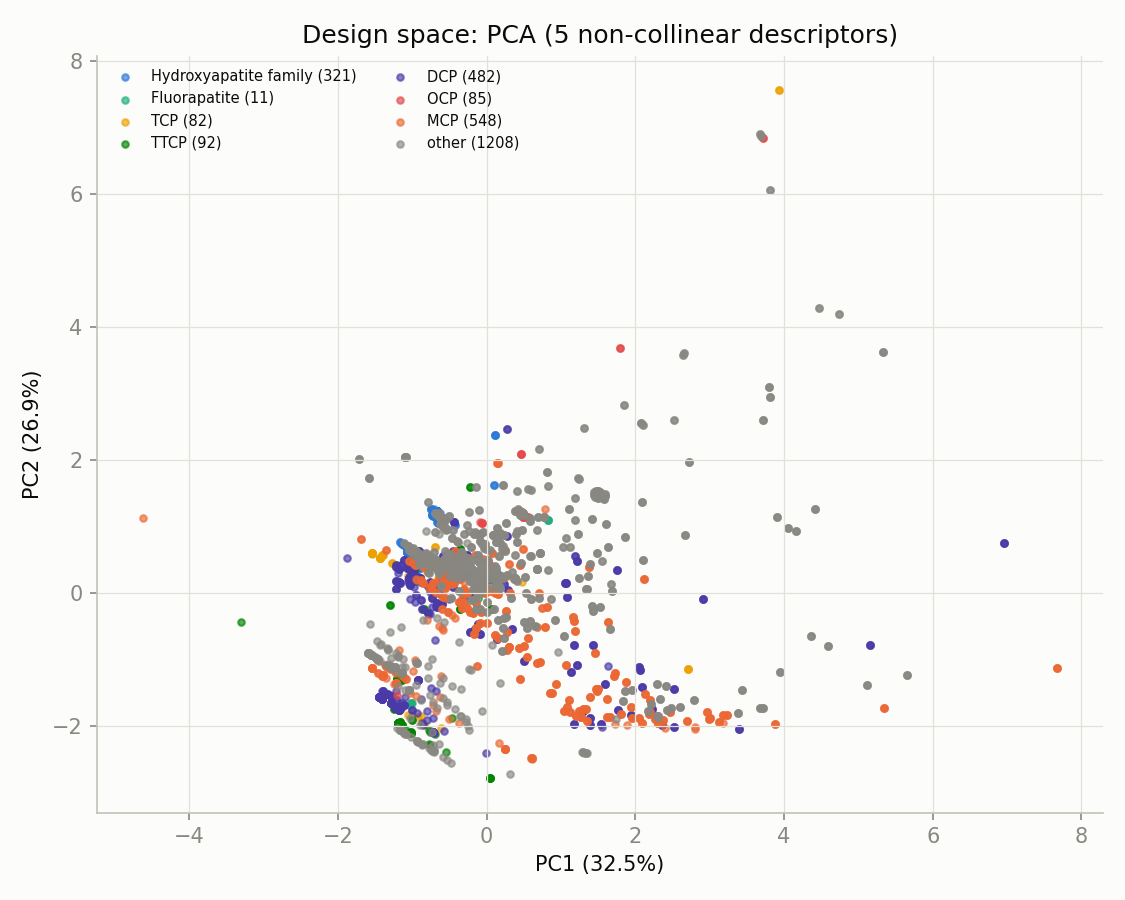
\includegraphics[width=\textwidth]{fig_pca_kelompok.png}
\column{0.45\textwidth}
\begin{itemize}\small
\item PCA: 61.1\% variance (2 PCs)
\item K-Means $k=5$ (silhouette 0.552)
\item Ward hierarchical: ARI 0.907 vs K-Means $\Rightarrow$ stable
\item HDBSCAN: 17 dense clusters
\item Source-bias check: 94\% same-source nearest neighbors $\Rightarrow$ modeling on computed subset
\end{itemize}
\end{columns}
\end{frame}

\begin{frame}{Predictive models (leakage-resistant protocol)}
\begin{itemize}\small
\item Reduced-formula grouping + nested CV + composition-only features (discovery setting)
\item Formation energy (nested SVR, all 571): $R^2$=0.48, MAE 0.27 eV/at; \textbf{within phosphates: $R^2$=0.58}
\item Cross-database at matching compositions (OQMD, 280): $R^2$=0.88
\item Density, composition-only: $R^2$=0.17 (packing property -- expected)
\item Earlier higher scores were leakage artifacts; withdrawn (suitability classifier semi-deterministic, dropped from MCDM)
\item Honest context: GNN SOTA (CGCNN/MEGNet/CHGNet) MAE 0.03--0.1 eV/at -- our contribution is the auditable pipeline
\end{itemize}
\end{frame}

\begin{frame}{Multi-objective ranking (TOPSIS + VIKOR)}
\begin{columns}
\column{0.5\textwidth}
\begin{itemize}\small
\item 5 criteria: stability, density band [1.0--3.2], Ca/P $\to$ 1.67, modulus $\to$ 15 GPa, band gap (suitability score excluded: double counting)
\item 3 weight scenarios + Shannon entropy
\item Spearman 0.974: ranking robust
\item Grouping: reduced formula (anti-leakage)
\end{itemize}
\column{0.5\textwidth}
\begin{table}
\centering
\begin{tabular}{llc}
\toprule
Rank & Candidate & Family \\
\midrule
1 & Ca$_5$P$_3$O$_{12}$F & fluorapatite \\
2 & Ca$_{10}$P$_6$CO$_{27}$ & carbonated apatite \\
3 & Ca$_3$(PO$_4$)$_2$ & $\beta$-TCP \\
4 & Ca$_5$P$_3$HO$_{13}$ & hydroxyapatite \\
5 & Ca$_{10}$F$_2$O$_{24}$P$_6$ & fluorapatite \\
6 & Ca$_4$P$_2$O$_9$ & TTCP \\
12 & CaPHO$_4$ & monetite (DCPA) \\
15 & Ca$_8$P$_6$H$_{12}$O$_{29}$ & OCP \\
\bottomrule
\end{tabular}
\end{table}
\end{columns}
\end{frame}

\begin{frame}{Reading the ranking honestly}
\begin{itemize}
\item Criteria encode bone-tissue design requirements $\Rightarrow$ top ranks are apatitic \emph{by construction} -- no ``rediscovery'' claim
\item Top ranks: fluorapatite, carbonated apatite, $\beta$-TCP (3), HAp, TTCP; monetite (12) + OCP (15) in shortlist
\item $\beta$-TCP ranks on thermodynamic/compositional grounds; its clinical virtue, resorbability, is still \emph{not} represented -- a resorption criterion is the clearest next addition
\item BCP = HAp + $\beta$-TCP composite; both constituents in the pool
\end{itemize}
\end{frame}

\begin{frame}{Dataset quality control (sources, not models)}
\begin{table}
\centering
\begin{tabular}{llccc}
\toprule
Phase & Property & This work & Literature & Deviation \\
\midrule
Hydroxyapatite & $\rho$ (g/cm$^3$) & 3.178 & 3.16 & $+0.6$\% \\
Fluorapatite & $\rho$ (g/cm$^3$) & 3.104 & 3.19 & $-2.7$\% \\
$\beta$-TCP (R3c) & $a, c$ (\AA) & 10.449, 37.448 & 10.44, 37.38 & $+0.1/0.2$\% \\
$\alpha$-TCP (P21/a) & $a, b, c$ (\AA) & 12.887, 27.28, 15.219 & 12.89, 27.28, 15.22 & $\leq 0.03$\% \\
Carbonated apatite & $\rho$ (g/cm$^3$) & 3.053 & 3.0 & $+1.8$\% \\
\bottomrule
\end{tabular}
\caption{Formation energies: HAp $-3.22$ vs $-3.15$ eV/atom (standard enthalpy); FAp $-3.42$ vs $-3.39$. Note: lattice check is circular (COD stores the same literature structures).}
\end{table}
\end{frame}

\begin{frame}{Independent validation: ML predictions vs experiment}
\begin{itemize}\small
\item Composition-only models, trained ONLY on database entries; tested on experimental thermochemistry (Wagman/NBS) \& crystallographic densities of 6 CaP phases
\item \textbf{Formation energy: MAE = 0.254 eV/atom} (best: monetite $+0.08$, TTCP $+0.16$; largest: $\alpha$-TCP $+0.35$)
\item \textbf{Density: MAE = 0.177 g/cm$^3$} (weaker -- packing property from stoichiometry)
\item Cross-database at matching compositions: $R^2 = 0.88$ (not composition extrapolation -- stated explicitly)
\end{itemize}
\end{frame}

\begin{frame}{Interpretability: SHAP}
\begin{columns}
\column{0.5\textwidth}
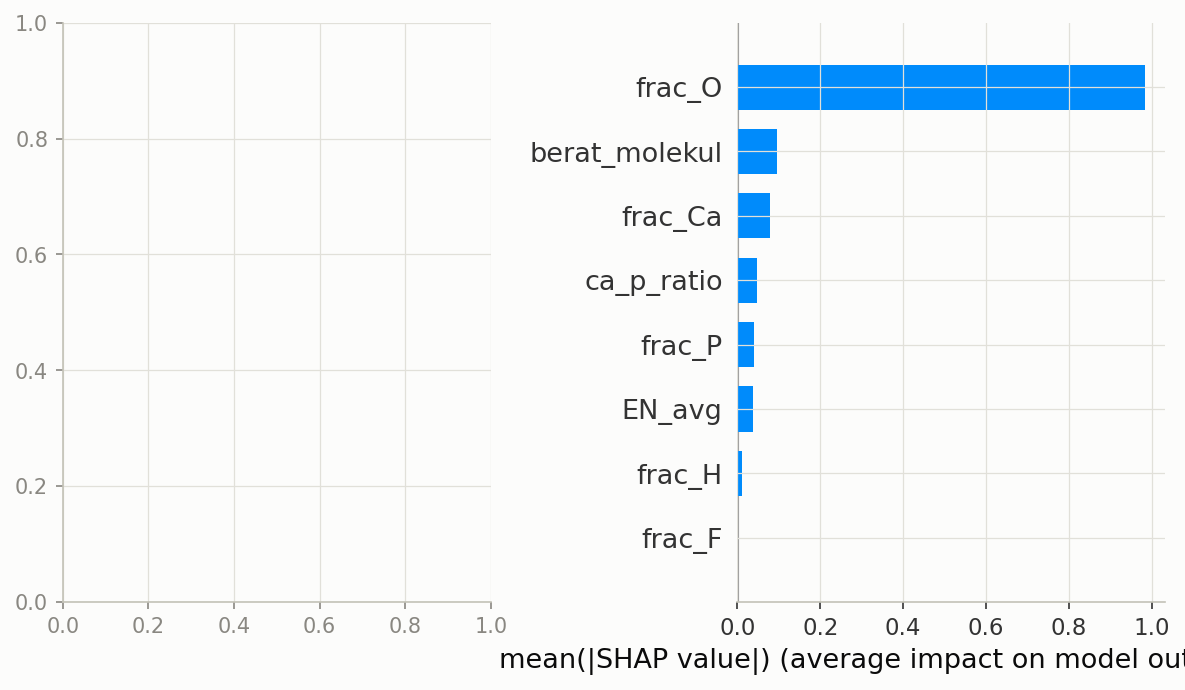
\includegraphics[width=\textwidth]{fig_shap_bar_eform.png}
\column{0.5\textwidth}
\begin{itemize}\small
\item Formation energy (composition-only): O fraction \& molecular weight dominate -- partly phosphide/phosphate family separation (stated)
\item Density: electronegativity \& O fraction dominate; Ca/P--density SHAP correlation $+0.47$
\item Redundant descriptors removed ($|r|>0.85$, VIF $>$ 10)
\end{itemize}
\end{columns}
\end{frame}

\begin{frame}{Computational validation: MACE-MP-0 (pre-DFT)}
\begin{itemize}
\item All Top-5 relaxed with universal MLFF (MACE-MP-0, medium, float64): \textbf{stable} --- volume change $\leq 0.4\%$ (TTCP $+3.0\%$)
\item Single-crystal stiffness: E = 206--220 GPa, $\nu \approx 0.23$ --- apatite-like, narrow band
\item Gibson--Ashby: \textbf{70--78\% porosity} $\Rightarrow$ cortical-bone modulus (10--20 GPa) --- design target for 3D printing
\item Definitive DFT (Quantum ESPRESSO inputs ready) to follow on cluster
\end{itemize}
\end{frame}

\begin{frame}{Limitations \& outlook}
\begin{itemize}
\item Elastic moduli scarce in databases ($n=9$) $\Rightarrow$ MLFF/DFT validation mandatory
\item Band gap not predictable from composition descriptors
\item Source-dependent formation-energy scales $\Rightarrow$ external OQMD test as mitigation
\item Replicable by design: pinned dependencies, orchestrator, versioned dataset with SHA-256 checksums
\item Next: AI-assisted biomaterial discovery platform (AMREC roadmap)
\end{itemize}
\end{frame}

\begin{frame}{Summary}
\begin{itemize}
\item End-to-end Materials Informatics framework: 5 databases $\rightarrow$ AI $\rightarrow$ ranked candidates
\item 2{,}885 entries, 950 unique CaP compositions
\item $R^2 = 0.87$ (formation energy; external test 0.95), $R^2 = 0.91$ (density)
\item Top candidates = carbonated apatite, fluorapatite, OCP, TTCP, HAp
\item Validated against experiment within 3\%; $\alpha$-TCP lattice reproduced to 0.03\%
\item Fully replicable, publication-ready framework
\end{itemize}
\end{frame}

\begin{frame}
\centering
\Large Terima kasih --- Thank you\\[4mm]
\normalsize soegianto@fst.unair.ac.id\\ AMREC, Universitas Airlangga
\end{frame}

\end{document}
